\chapter{Operating System Overview 2}
I dette kapittelet skal du lære:\newline \newline
$\text{\rlap{$\checkmark$}}\square$
Summere opp hovedfunksjoner til et operativ system. \newline \newline
$\text{\rlap{$\checkmark$}}\square$ 
Diskutere utviklingen til OS fra batch system til nyere komplekse OS. \newline \newline
$\text{\rlap{$\checkmark$}}\square$ 
Kort oppsumering av OS forskning. \newline \newline
$\text{\rlap{$\checkmark$}}\square$ 
Diskutere hoved-design-områdene i utvikling av OS. \newline \newline
$\text{\rlap{}}\square$ 
Definere virituelle maskiner og virituallisering. \newline \newline

\section{Operativsystem}
Et operativsystem er et program som styrer "execution" av andre applikasjoner. Det er et "interface" mellom hardware og software.
\newline \newline
For å modelere strukturen mellom hardware og software så bør du titte på figur \ref{fig:computerHS}. Brukeren av en datamaskin vil stortsett ikke måtte tenke på detaljer i hardware strukturen. Brukeren ser på datasystemet som et set med applikasjoner. Applikasjonen er øverst, eterfulgt av bibloteker og drivere, så opperativsystemet som har kontakt med execution hardware. Hardware kontrollerer minne overføring, (Memory translation) og system tilkobliner (bus). Som igjen har kontakt med I/O devices og network, sammen med main memory.\newline\newline

\begin{figure}[h]
\centering
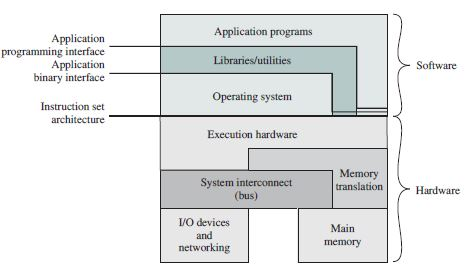
\includegraphics{img/ComputerHS.JPG}
\caption{Layers in Hardware Software structure}
\label{fig:computerHS}
\end{figure}

Et operativsystem brukes til følgende oppgaver :
\begin{itemize}
\item Program development
\item Program execution
\item Access I/Odevices
\item Controlled access to files
\item System access.
\item Error detection and response
\item Accointing
\end{itemize}
~\\
\subsection{Interfacing the OS}
Interface til OS skjer gjennom.
\begin{itemize}
\item Instruction set architecture (ISA)
\item Application binary interface (ABI)
\item Application programming interface (API)
\end{itemize}
\subsubsection{API}
Der for oss dødelige så er API den mest kjente av disse hovedgruppene. 
Tenk på API som en programmerers tilgang til all hardware. Si du har lyst å benytte deg av en "feature", feks et biblotek eller operativsystemet så vil du bruke API. Et API består av datatyper/strukturer, constanter, funksjoner, etc som du kan bruke i din kode for å aksessere funksjonaliteter til eksterne komponenter.
\subsubsection{ABI}
Et ABI er veldig likt, tenk på det som den kompilerte versjonen av et API (eller som et API på maskin-språk nivå). Når du skriver kildekode, aksesseres bibloteket gjennom et API. Med en gang koden er kompilert, så aksesseres den binære data i bibloteket gjennom et ABI.
\subsubsection{ISA}
ISA er den delen av prosessoren som er synlig for programmereren eller kompliatoren. ISA fungerer som en grense mellom software og hardware. Du kjenner kanskje til ARM, INTEL, AVR, og lignende. Dette er instruksjonsettene, som gjør ca det samme, men er likevell ganskje forskjellige. Du kan ikke kjøre windows 98 på en ARM prosessor, og du kan ikke kjøre Android på en intel prosessor.

\section{Operativsystem som Resource Manager}
En datamaskin er et set med ressurser for å flytting, lagring, og prossesering av data og for å kontrollere disse funksjonene. OS har ansvar for og håndtere alle disse ressursene. 
Operativsystemet fungerer riktignok ikke helt som kanskje forventet. På en side er det en program av programmer som utføres av prosessoren. 
På en annen side må prosessoren hele tiden gi fra seg kontrollen og forholde seg til når prosessoren gir tilbake kontrollen. 
Hovedforskjellen fra et OS til et program er at for å klare å kjøre andre programmer må den slutte å jobbe selv og la prosessoren gjøre noe "nyttig" arbeid. Etter dette "nyttige" arbeidet er utført tar den over i lang nok tid til å forberede prosessoren for et nytt stykke arbeid. 

\subsection{Oppbygning}
En liten porsjon av OS ligger i hovedminne, det inkluderer \emph{kernelen} som inneholder de mest frekvente funksjonene til OS, og ved gitt tid, andre deler av OS som er i bruk. Hardware sin minnehåndtering i prosessoren og OS kontrollerer sammen allokering av minne. OS bestemmer også hvilke program som får tilgang til I/O devices. Prosessoren selv er en ressurs, og OS må avgjøre hvor mye tid et enkelt program får med prosessoren. Ved flere prosessorer (multiprosessor) så må avgjørelsen spenne over alle prosessorene. 
\section{Utvilkingen av Operativsystemet}
Et OS vil utvikle seg over tid av ulike årsaker.
\begin{itemize}
\item \emph{Hardware oppgradering, og nye typer hardware:} For eksempel tidlige versjoner av UNIX og Macintosh OS hadde ikke støtte for paging, fordi de ble kjørt på prosessorer uten paging støtte. 
\item \emph{Nye brukerbehov:} Når brukere krever mer, for eksempel hvis det er vanskellig å oppnå god performance med de verktøy som finnes.
\item \emph{Fixes:} Ethvert OS har feil, de må oppdateres.
\end{itemize}

I gamle dager 1940 - 1950,så var datamaskinene uten OS. En bruker satt av tid typisk 1 time etc, for å benytte seg av datamaskinen. Her var det lett å enten bruke for lite, eller for mye av tiden og det endte med enten bortkastet computer, eller at alt arbeidet var forgjeves pga for lite tid.
Les mer om de gamle pcene i Stallings side 53.
\subsection{Simple Batch System}
Pga bortkastet datakraft begynte IBM med noe som de kalte Simple Batch System. Her er ideen og bruke en bit i software, kalt \emph{monitor}, der brukeren ikke lenger hadde direkte tilgang på prosessoren. Monitoren leser en jobb av gangen, plaserer det i program området, og forlater kontrollen over prosessoren. Når jobben er ferdig så tar monitoren over prosessoren igjen. Ganske så smart.
Et batch system er bare et program, den er avhengig av at prosessoren gir tilbake kontrollen og noen features er ønsket. 
Feks, skulle et program prøve å endre områede der monitoren er plasert i minne, må prosessoren stoppe dette og avbryte. Et annet scenario er "timer", hvis et program bruker for mye tid. I tilegg har vi priviligerte instruksjoner for monitoren, og interrupts.

\section{Multiprogrammering av Batch System}
Selv nå som jobben gjøres automatisk i forhold til de gamle pcen på 1940 - 1950, så viste det seg at prosessoren som er superrask relativt til I/O devices, kastet bort tid. Typisk hentet vi en "record" fra fil 15$\mu s$, utførte 100 instruksjoner 1$\mu s$, og skrev tilbake "record" til fil 15$\mu s$. 

Hvis vi derfor tillater at mens en I/O modul laster så kjører vi et annet program i mellomtiden så kan vi oppnå bedre utilisasjon. Her kommer naturligvis scheduling in som vi skal snakke om senere. 

Ta for eksempel programmene i figur \ref{fig:utilization}. Ved å bruk av multiprogramming som i figur \ref{fig:multiprog}, kan man oppnå en mye bedre total kjøretid for alle tre programmene. 
\begin{figure}
\centering
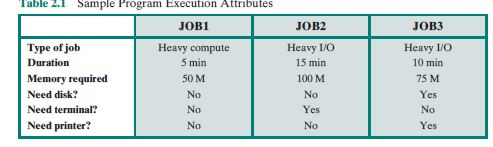
\includegraphics{img/utilization.JPG}
\caption{Programmer og kjøretid}
\label{fig:utilization}
\end{figure}
\begin{figure}
\centering
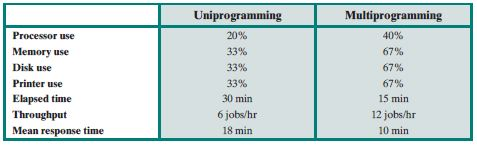
\includegraphics{img/multiprogramming.JPG}
\caption{Kjøretider}
\label{fig:multiprog}
\end{figure}

Den største ekstra featuren som er verdt og nevne i sammenheng med multiprogramming er hardware som støtter interrupt, og \href{https://en.wikipedia.org/wiki/Direct_memory_access}{DMA}. 
\section{Time-Sharing System}
I dag har mange sin egen datamaskin, i gamle dager hadde man ikke det, så de oppfant "time-sharing". Det handlet rett og slett om å dele prosessortiden. Flere brukere jobbet i terminalen samtidig, og prosessoren byttet raskt imellom dem. Hver bruker fikk da $1/n$ tid med prosessoren, uten å regne med OS overhead. Men gitt at en bruker ikke reagerer så raskt så vil ikke brukeren oppleve forskjell. I denne sammenhengen kommer order \emph{Time-Slicing}, typisk hvert 0.2 sekund fikk prosessoren et interrupt og OS tok over. Da kunne OS tilsette en ny bruker den ønskede oppgaven. Den gamle brukeren sitt program blir lastet ut på disk og den nye brukerens program blir lastet inn. Forskjellen mellom Batch Multiprogramming og Time-Sharing kan sees i tabell \ref{fig:batchvstime}
\begin{figure}
\centering
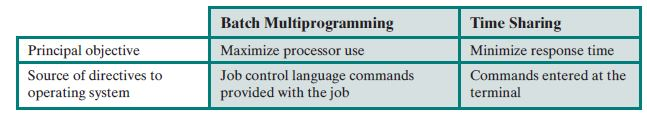
\includegraphics{img/batchvstime.jpg}
\caption{Batch multiprogramming vs Time-Sharing}
\label{fig:batchvstime}
\end{figure}

\section{Major Acheivements}
Fordi et OS er muligens et av de mest komplekse software formene du kan få tak i så er det begreper som er sentrale for å kunne forklare utviklingen av OS.
\begin{itemize}
\item Process
\item Memory Management
\item Information protection security
\item Scheduling and resource management
\end{itemize}

Dette kan være viktig å definere på eksamen så la oss hoppe inn i det.
\subsubsection{The Process}
Begrepet ble først brukt... Hvem bryr seg. Det er et mer generelt begrep en "job". Det finnes flere definisjoner som: et program i en "execution", eller en instans av et program på en computer. Det er også definert som "The entity that can be assigned to and executed on a computer", eller "A unit of activity charictar... jaja kommer ikke til å huske uanset. Mer forståelse kommer. 
\newline\newline
Som vi nettop ble kjent med så var målet med multiprogrammering og holde orden på lagring, I/O devices, og prosessoren for å maksimere effektiviteten. 
Det viste seg å være ganske vanskellig, og error som oppstod ble veldig harde å reprodusere. I det generelle hadde man fire typer error:
\begin{itemize}
\item Improper synchronization, det er ikke uvanlig at en rutine må vente på at noe annet i systemet skal bli ferdig. Eksempelvis kunne man la være å vente på at data var ferdig i buffer og signalet som egentlig skulle bli sendt ble aldri mottat.
\item Failed mutual exclution, feks, to brukere som prøver å aksessere samme fil samtidig. 
\item Nondeterminate program operation, resultatet i et program burde være kun avhengig av input, men når flere programmer deler minne/prosessor, kan det fortsatt hende at programmene overskriver delt minne uten konfirmasjon fra det andre programmet. 
\item Deadlocks, dette her burde være kjent fra tidligere. Google if not.
\end{itemize}

Det som trengs for å takle disse problemene er en systematisk måte å monitorere og kontrollere program som kjøres i prosessoren. Vi kan tenke på at en prosess består av tre komponenter:
\begin{itemize}
\item Et "executable program"
\item Den assosierte data, som trengs av programmet (variabler, arbeidsområede, buffer).
\item "The execution context of the program" konteksten altså.
\end{itemize}
Den siste \emph{"The execution context of the program"} er essensiell. Den er kjent som \emph{process state}, og er intern data som OS er i stand til å overvåke. Denne interne data er separert fra OS.  
I konteksten finnes alt OS trenger for å håndtere prosessen, her finner du prosessor registere, feks PC og data registere. Den inneholder også nyttig data som prioritet, og om den venter på fullføring av I/O event.
\subsection{Virituelt minne}
Dette er et kort utdrag fra Memory management. Det handler om at vi må isolere prosessene fra å ødelegge for hverandre (data og instruksjoner). Programmer burde derfor allokeres dynamisk over minne hierarkiet. Allokering bør være transparant for programmereren, derav virituelt minne. Effektiviteten økes når OS assigner minne til bare de jobbene som trenger det. 
Fordi minnekravet er varierende over forskjellige prosesser så ble \emph{paging} introdusert. Viktig del å kunne litt om det der. Prosessene ble tillat og inneholde et antal avsatte blokker (blocks) som kalles pages. En programmere reffererer ererer... til ord (words) i form av \emph{virtual adress} som består av en "page number" og en offset innenfor "the page". Etter dette ble inført ble neste oppgave å tillate at minne ikke lenger måtte ligge i samme hovedminne samtidig.  